\documentclass{standalone}
\usepackage{ tikz }
\usepackage{ xparse }
\input{macros/all}

\begin{document}

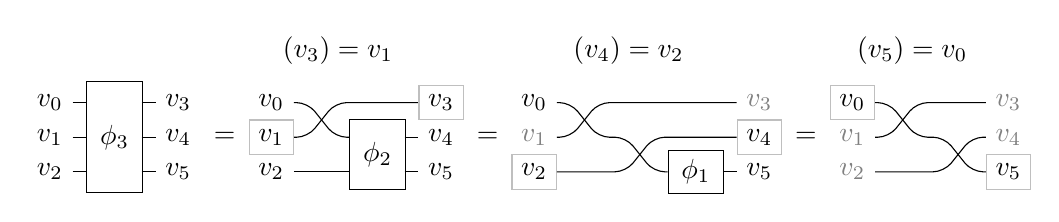
\begin{tikzpicture}[yscale = -1, x = 0.5em, y = 1.25em]

    %step1

    \draw[rounded corners] (1,1) -- (2,1);
    \draw[rounded corners] (1,2) -- (2,2);
    \draw[rounded corners] (1,3) -- (2,3);
    
    \node[minimum width=1em,minimum height=1em,anchor=east] at (1,1){$v_0$};
    \node[minimum width=1em,minimum height=1em,anchor=east] at (1,2){$v_1$};
    \node[minimum width=1em,minimum height=1em,anchor=east] at (1,3){$v_2$};

    \node[draw,minimum width=2em, minimum height = 4em, anchor=west] at (2,2){$\phi_3$};

    \draw[rounded corners] (6,1) -- (7,1);
    \draw[rounded corners] (6,2) -- (7,2);
    \draw[rounded corners] (6,3) -- (7,3);

    \node[minimum width=1em,minimum height=1em,anchor=west] at (7,1){$v_3$};
    \node[minimum width=1em,minimum height=1em,anchor=west] at (7,2){$v_4$};
    \node[minimum width=1em,minimum height=1em,anchor=west] at (7,3){$v_5$};

    \node at (12,2){$=$};

    %step2 

    \draw[rounded corners] (17,1) -- (18,1) -- (20,2) -- (21,2);
    \draw[rounded corners] (17,2) -- (18,2) -- (20,1) -- (26,1);
    \draw[rounded corners] (17,3) -- (18,3) -- (20,3) -- (21,3);

    \node[minimum width=1em,minimum height=1em,anchor=east] at (17,1){$v_0$};
    \node[draw = lightgray, minimum width=1em,minimum height=1em,anchor=east] at (17,2){$v_1$};
    \node[minimum width=1em,minimum height=1em,anchor=east] at (17,3){$v_2$};

    \node[draw,minimum width=2em, minimum height = 2.5em, anchor=west] at (21,2.5){$\phi_2$};

    \draw[rounded corners] (25,2) -- (26,2);
    \draw[rounded corners] (25,3) -- (26,3);

    \node[draw = lightgray, minimum width=1em,minimum height=1em,anchor=west] at (26,1){$v_3$};
    \node[minimum width=1em,minimum height=1em,anchor=west] at (26,2){$v_4$};
    \node[minimum width=1em,minimum height=1em,anchor=west] at (26,3){$v_5$};

    \node[anchor=west] at (15.5,-0.5) {$\vconnsl(v_3) = v_1$};

    % step3

    \node at (31,2){$=$};

    \node[minimum width=1em,minimum height=1em,anchor=east] at (36,1){$v_0$};
    \node[text = gray, minimum width=1em,minimum height=1em,anchor=east] at (36,2){$v_1$};
    \node[draw = lightgray, minimum width=1em,minimum height=1em,anchor=east] at (36,3){$v_2$};

    \draw[rounded corners] (36,1) -- (37,1) -- (39,2) -- (40,2);
    \draw[rounded corners] (40,2) -- (41,2) -- (43,3) -- (44,3);
    \draw[rounded corners] (36,2) -- (37,2) -- (39,1) -- (49,1);
    \draw[rounded corners] (36,3) -- (41,3) -- (43,2) -- (49,2);

    \node[draw,minimum width=2em, minimum height = 1em, anchor=west] at (44,3){$\phi_1$};

    \draw[rounded corners] (48,3) -- (49,3);

    \node[text = gray, minimum width=1em,minimum height=1em,anchor=west] at (49,1){$v_3$};
    \node[draw = lightgray, minimum width=1em,minimum height=1em,anchor=west] at (49,2){$v_4$};
    \node[minimum width=1em,minimum height=1em,anchor=west] at (49,3){$v_5$};

    \node at (54,2){$=$};

    \node[anchor=west] at (36.5,-0.5) {$\vconnsl(v_4) = v_2$}; 

    %step4

    \node[draw=lightgray, minimum width=1em,minimum height=1em,anchor=east] at (59,1){$v_0$};
    \node[text=gray,minimum width=1em,minimum height=1em,anchor=east] at (59,2){$v_1$};
    \node[text=gray,minimum width=1em,minimum height=1em,anchor=east] at (59,3){$v_2$};

    \draw[rounded corners] (59,1) -- (60,1) -- (62,2) -- (64,2) -- (66,3) -- (67,3);
    \draw[rounded corners] (59,2) -- (60,2) -- (62,1) -- (67,1);
    \draw[rounded corners] (59,3) -- (64,3) -- (66,2) -- (67,2);


    \node[text=gray,minimum width=1em,minimum height=1em,anchor=west] at (67,1){$v_3$};
    \node[text=gray,minimum width=1em,minimum height=1em,anchor=west] at (67,2){$v_4$};
    \node[draw = lightgray, minimum width=1em,minimum height=1em,anchor=west] at (67,3){$v_5$};

    \node[anchor=west] at (57, -0.5){$\vconnsl(v_5) = v_0$};
\end{tikzpicture}

\end{document}